\chapter{Proposta}
\label{chapter:Proposta}

A seguir será detalhado cada ponto proposto em tópicos mais detalhados, visando especificar cada fragmento que será desenvolvido no decorrer deste trabalho.

Ao final deste capítulo será possível ter uma ideia concreta da proposta deste trabalho e do principal funcionamento do \textit{framework}.

\section{O Framework}

A proposta deste trabalho é desenvolver um \textit{framework} que auxilie no desenvolvimento de redes sociais. Este \textit{framework} deve oferecer recursos gerais com toda a lógica de usuários e relacionamentos, e recursos mais específicos para redes sociais baseadas em rotas e agendas. O recurso de rotas deve ser capaz de fazer um mapeamento de trajetos de interesse de um determinado usuário e auxiliar este a fazer comparações com rotas de outros usuários. A agenda deve oferecer recursos de controle de ocupações no decorrer de dias e horários e auxiliar um usuário a encontrar dias e/ou horários comuns entre um grupo de usuários qualquer.

Todo o \textit{framework} será extensível de forma que será possível que o desenvolvedor, a partir de heranças, consiga acrescentar e ou mudar implementações conforme as suas necessidades. Porém, o \textit{framework} por si só já irá oferecer recurso variados e completos que darão ao desenvolvedor a possibilidade de criação de uma rede social completa sem a necessidade de realização de quaisquer alterações no que é fornecido, a extensibilidade só é necessária quando se chega a algumas especificidades da aplicação que não são fornecidas.

A seguir têm-se um maior detalhamento de cada um dos três principais componentes fornecidos pelo \textit{framework}.

\subsection{Relacionamento de Usuários}

O relacionamento em redes sociais dá-se por meio de interações entre os usuários. Estas interações variam de acordo com a rede em que o usuário está inserido. Alguém pode apenas seguir outras pessoas e acompanhar suas postagens, este é um relacionamento unidirecional, pois não é necessário que uma pessoa seguida acompanhe também postagens de seus seguidores. Existe também outro tipo de relacionamento, onde é necessário que as duas pessoas estejam diretamente ligadas entre si, o que o torna necessariamente bidirecional. Neste tipo pode-se considerar relacionamentos entre conhecidos, amigos, namorados, familiares, entre outros.

Na montagem da estrutura de relacionamentos entre os usuários para redes sociais, é necessário fazer uso de grafos, onde os usuários serão representados como os vértices e os relacionamentos como as arestas. No caso dos relacionamentos unidirecionais, apenas uma aresta é criada. Esta aresta faz uma ligação a partir do vértice do usuário seguidor para o vértice do usuário que este deseja seguir, como pode ser observado na Figura \ref{segue}. No caso dos relacionamentos bidirecionais, a ligação deverá ser feita usando-se duas arestas paralelas. É necessário que para ambos os usuários exista uma possibilidade de se chegar ao outro, portanto, deve existir uma aresta que ligue um usuário ``A'' a um usuário ``B'' e uma aresta que ligue o usuário ``B'' ao usuário ``A'', vide a Figura \ref{amigo}.

\begin{figure}[!h]
	\centering
	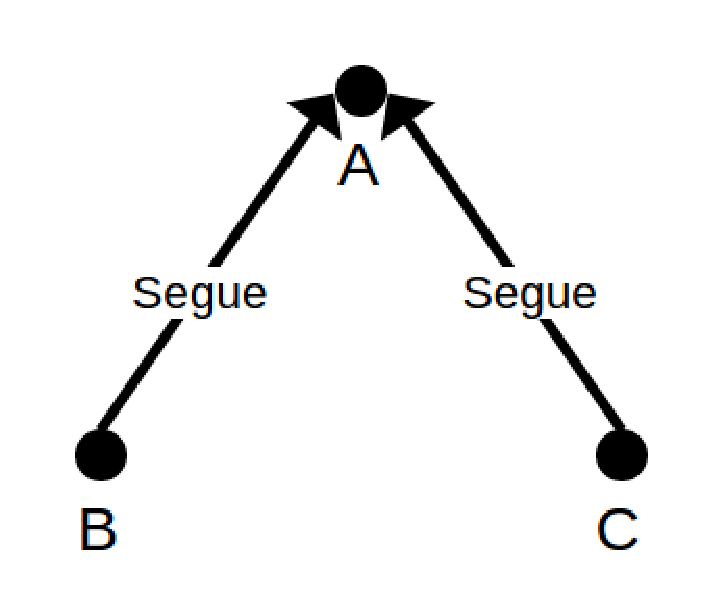
\includegraphics[scale=0.45]{figuras/capitulo5/segue.eps}
	\caption{Exemplo de aresta de seguir usuário}
	\label{segue}
\end{figure}

\begin{figure}[!h]
	\centering
	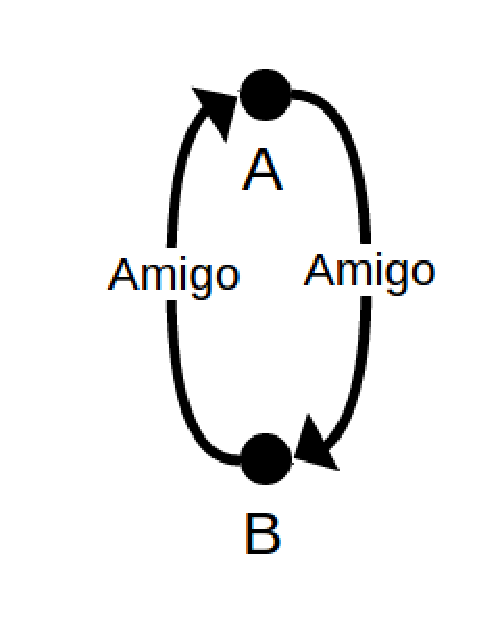
\includegraphics[scale=0.45]{figuras/capitulo5/amigo.eps}
	\caption{Exemplo de arestas pararelas de amizade}
	\label{amigo}
\end{figure}

Cada aresta deverá possuir uma ou mais descrições que detalham qual o relacionamento entre os usuários. Isso fica mais claro ao se falar de relacionamentos bidirecionais, onde pode existir entre duas pessoas um relaciomanento de amizade e parentesco, por exemplo. Esse relacionamento pode ser visualizado na Figura \ref{parentes}.

\newpage

\begin{figure}[!h]
	\centering
	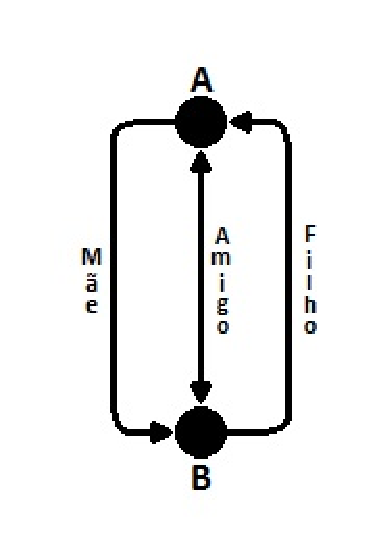
\includegraphics[scale=0.45]{figuras/capitulo5/parentes.eps}
	\caption{Exemplo de arestas pararelas parentesco}
	\label{parentes}
\end{figure}

\subsection{Controle de Rotas}

Rota\footnote{\url{http://www.dicio.com.br/rota/}} é um itenerário que se percorre para ir de um lugar a outro, indicando a direção ou rumo a ser percorrido, Um exemplo de rota pode ser visualizado na Figura \ref{rota}.

\begin{figure}[!h]
	\centering
	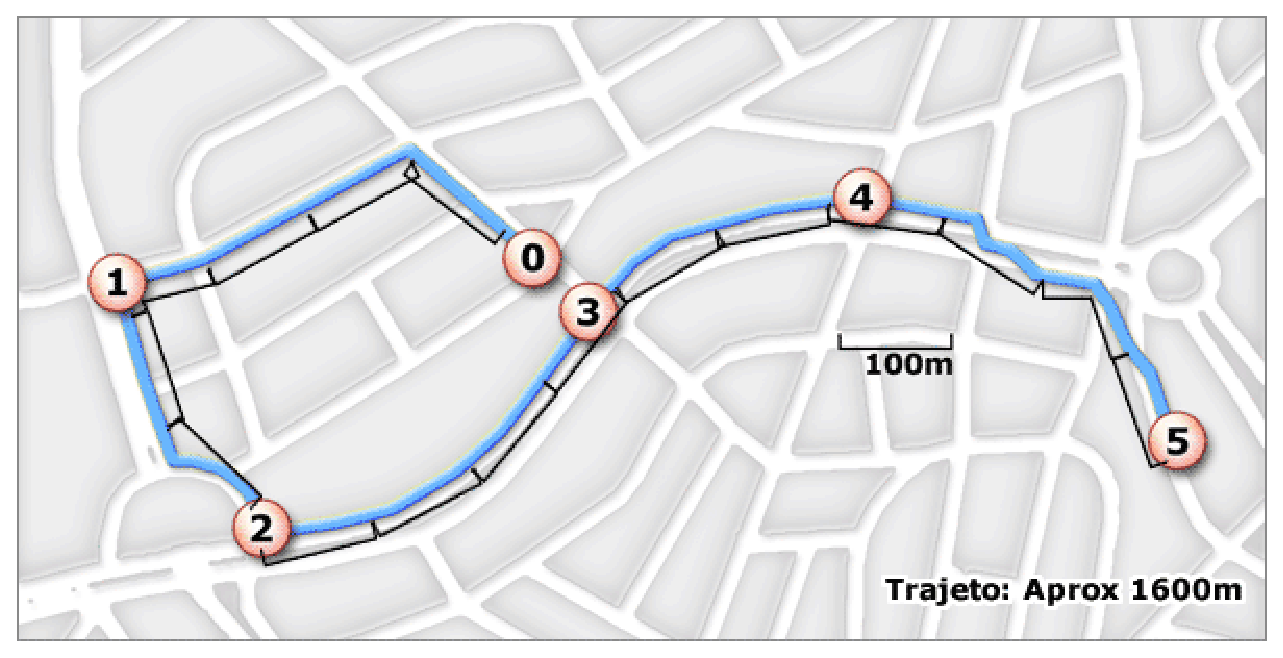
\includegraphics[scale=0.55]{figuras/capitulo5/rota.eps}
	\caption[Exemplo de rota]{Exemplo de rota\footnotemark}
	\label{rota}
\end{figure}
\footnotetext{\url{http://sede.wikidot.com/andy-s-brainstorm}}

O \textit{framework} irá oferecer recursos que auxiliem o usuário a definir as rotas que percorre e os horários de cada percurso, e buscar rotas de outros usuários que coincidam em parte ou integralmente com as suas.

Redes socias podem utilizar estes dados para aplicações diversas como, por exemplo, caronas e encontros para ciclistas.

Conforme mostrado na figura \ref{rota}, pode-se ver uma rota que leva do ponto ``0'' ao ponto ``5'', poderiam existir diversos usuários com rotas comuns nesse caminho, por exemplo, um usuário que siga todo o caminho traçado, ou um usuário que partisse do ponto ``2'' e chegasse ao ponto ``4'' e assim por diante. Uma das funcionalidades do \textit{framework} neste contexto seria encontrar todos os usuários que partilhassem desses caminhos em comum, ou encontrar um caminho partilhado entre um grupo de usuários, por exemplo.

\subsection{Controle de Agenda}

Outra funcionalidade que o \textit{framework} irá fornecer é a conciliação de agendas entre os usuários, possibilitando assim encontrar dias da semana e horários específicos que são comuns a um determinado grupo. Esta funcinalidade pode auxiliar os usuários em diversos aspectos como, por exemplo, encontrar um horário em comum para realizar uma tarefa.

A figura \ref{agenda semanal} mostra um exemplo de uma agenda semanal com todos os horários livres.

\begin{figure}[!h]
	\centering
	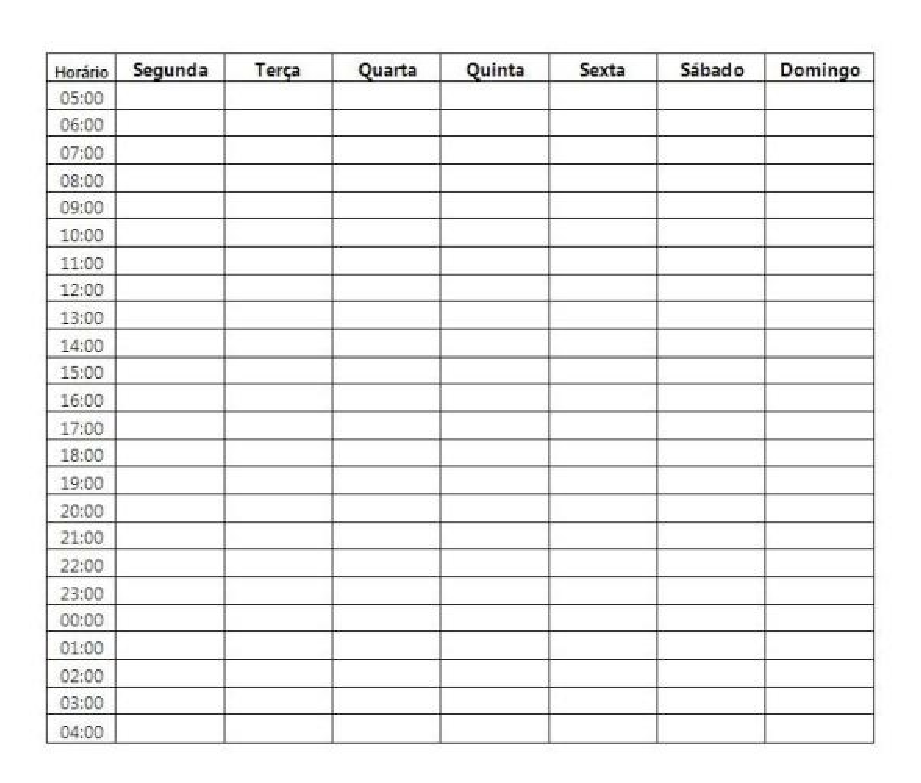
\includegraphics[scale=0.55]{figuras/capitulo5/agenda_semanal.eps}
	\caption[Exemplo de agenda semanal]{Exemplo de agenda semanal\footnotemark}
	\label{agenda semanal}
\end{figure}
\footnotetext{\url{http://universovocesaude.com.br/wp-content/uploads/2014/08/horario-semanal_JPG.jpg}}

Agendas dessa forma auxiliam usuários a terem um melhor controle de suas tarefas semanais, marcarem eventos, entre outros aspecetos. O período compreendido por uma agenda pode variar de acordo com cada contexto, uma agenda semanal conforme a apresentada, mensal, anual, ou ainda um período não necessariamente pré-definido, o que poderia auxiliar usuários a marcarem eventos para longas datas futuras. De modo simplificado, basta dados como dia e horários de início e fim de uma tarefa para aplicar um controle de agenda.

O \textit{framework} oferecerá o suporte para criação de agendas conforme apresentado, assim, é possível a partir de um período pré-determinado encontrar um horário e dia comuns a um conjunto de usuários, isso pode auxiliar a criação e marcação de enventos visando atender o maior número de usuários conforme o contexto da aplicação.

\subsection{Modelo Inicial}

A Figura \ref{diagrama de componentes} apresenta os principais componentes que serão oferecidos pelo \textit{framework}. Fica evidenciado, no modelo, o relacionamento de usuário com rotas e agendas. Em cada um desses componentes, existirão diversas classes que implementarão todo o modelo e as regras de negócio propostas.

\begin{figure}[!h]
	\centering
	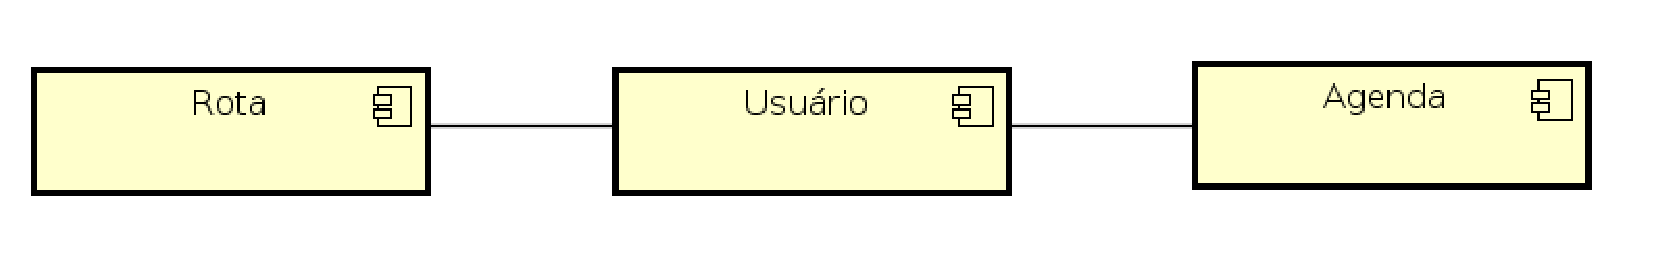
\includegraphics[scale=0.55]{figuras/capitulo5/diagrama_componentes.eps}
	\caption{Diagrama de componentes inicial}
	\label{diagrama de componentes}
\end{figure}

Este modelo servirá como base para a implementação de todas as funcionalidades propostas.

\section{Uso do Framework}

O \textit{framework} será desenvolvido em \textit{``Ruby on Rails''} e terá sua \textit{``Gem''}\footnote{\url{http://www.akitaonrails.com/2009/2/2/entendendo-rubygems}} publicada em um repositório \textit{online} para uso de outros desenvolvedores.

Para comprovação do funcionamento do \textit{framework}, este trabalho propõe o desenvolvimento de uma rede social que faça uso do mesmo. Esta rede deverá fazer uso dos principais recursos providos pelo \textit{framework}, dessa forma, pode-se ver o seu uso na prática.

\section{Prova de Conceito}

Foi desenvolvida uma aplicação simples para implementação de alguns conceitos discutidos neste trabalho.

De modo geral, a aplicação desenvolvida implementa uma rede de usuários ligados entre si formando um grafo. A solução contêm com as classes Usuário, Aresta e Grafo. A classe Aresta é usada para fazer as ligações entre as entidades. A classe Grafo representa a própria rede com todos os usuários. Foram implementadas as funcionalidades de relacionamento descritas nas Figuras \ref{segue} e \ref{amigo}, além de uma varredura dos usuários presentes no grafo pelos algoritmos de busca ~\nameref{subsec:bfs}, \textit{Breadth-First Search}, e ~\nameref{subsec:dfs}, \textit{Depth-First Search}.

Todo o código fonte da aplicação citada pode ser encontrado em \url{https://github.com/TCC-SocialNetwork/concept-test}.

Essa aplicação representa a prova de conceito visando entender detalhes básicos de redes sociais, e compreender as reais dificuldades para o pleno desenvolvimento do \textit{framework} proposto. Essa prova de conceito procura lidar com uma funcionalidade chave em redes sociais, no caso, o relacionamento de usuários. Portanto, é vista como um passo inicial para o desenvolvimento da proposta. O desenvolvimento completo será realizado na segunda parte deste trabalho, conforme evidenciado no fluxo de trabalho bem como no cronograma, ambos apresentados no capítulo de ~\nameref{chapter:Metodologia}.

\section{Trabalhos Relacionados}

Em algumas pesquisas relacionadas sobre trabalhos parecidos com o que se propõe, pode-se encontrar alguns sistemas semelhantes, os quais serão apresentados a seguir..

Existe uma comparação entre vinte e cinco plataformas, plataformas, as quais colaboram para começar um serviço de rede social\footnote{\url{http://www.tripwiremagazine.com/2010/07/25-best-social-networking-platforms-to-start-your-own-service.html}}  próprio. Porém, a  maioria das plataformas apresentadas é paga ou não é voltada para desenvolvedores, ou seja, são plataformas que fornecem funcionalidades para usuários comuns poderem montar uma rede social a partir de um \textit{template} visual já definido.

\begin{table}[]
\centering
\caption{My caption}
\label{my-label}
\begin{tabular}{@{}llllll@{}}
\toprule
\textbf{Rede Social}  & \textbf{Licença} & \textbf{Preço}        & \textbf{Linguagem}  & \textbf{Customizável}                                    & \textbf{Instalação} \\ \midrule
SocialEngine          & Customizada      & A partir de \$ 299,99 & PHP                 & Sim                                                      &                     \\
Elgg                  & GPL 2.0          & Grátis                & PHP                 & Extensível via plugins e com uma API flexível            &                     \\
XOOPS                 & GPL 2.0          & Grátis                & PHP                 & Extensível via módulos                                   &                     \\
Anahita Social Engine & GPL 2.0          & Grátis                & PHP                 & Sim                                                      &                     \\
Telligent Community   & Customizada      & Grátis com limitações & ASP .NET            & Extensível via plugins, widgets, tarefas, eventos e REST &                     \\
Newebe                & AGPL             & Grátis                & Python/Coffeescript & Sim                                                      &                     \\
Buddycloud            & Apache 2.0       & Grátis                & NodeJS/Java         & Não*                                                     &                     \\
eXo Platform          & LGPL             & Grátis                & Java                & Extensível via plugins e com uma API flexível            &                     \\
Kune                  & AGPLv3           & Grátis                & Java                & Extensível via widgets e módulos                         &                     \\
Diaspora              & AGPLv3           & Grátis                & Ruby                & Sim                                                      &                     \\
Libertree             & AGPLv3           & Grátis                & Ruby                & Não*                                                     &                     \\ \bottomrule
\end{tabular}
\end{table}

Existem também alguns \textit{frameworks} mais semelhantes desenvolvidos em \textit{Ruby}\footnote{\url{https://www.ruby-toolbox.com/categories/social_networking}}. Estes, em sua maioria, fornecem recursos a desenvolvedores porém apenas a parte geral de relacionamento de usuários.

\section{Resumo do Capítulo}

Este capítulo concretizou a proposta deste trabalho apresentando seus pontos principais e alguns detalhes técnicos.

A partir desse escopo inicial, pretende-se desenvolver um \textit{framework}  capaz de auxiliar interessados no desenvolvimento de redes sociais, das funcionalidades básicas às específicas dos domínios de rota e agenda. Dando continuidade aos resultados obtidos até o momento, com a prova de conceito, serão elaborados os requisitos detalhados para construção do \textit{backlog} do produto e, a partir desse a definição das \textit{sprints} e \textit{releases} que existirão durante o desenvolvimento.

O próximo capítulo fecha este documento com uma conclusão parcial de todo o trabalho feito até o presente momento. Este capítulo deverá ser incrementado após a finalização da etapa de desenvolvimento do \textit{framework}.
